\chapter{Fundamentals}
\label{chap:ner-overview}

This chapter aims to give the reader a basic overview about the idea behind \acrlong{ner}, the expected benefits for Swiss Mobiliar, and information about the state of the art. General difficulties and the solutions to these problems are mentioned as well.

\section{A Brief Overview}

\acrshort{ner} is a subtask of information extraction. It seeks to find named entities (\acrshort{ne}) in unstructured text and classify them into predefined categories such as person names, locations, and organisations. A \acrlong{ne} is a real-world object with a proper name like \emph{Roger Federer}, \emph{New York City}, or the \emph{catholic church} \cite{wiki02}. Table \ref{tbl:named-entities} shows typical \acrlong{ne} types which are supported by a large variety of \acrshort{ner} libraries. Sometimes this group is extended with types like prices, dates, and times \cite{Jurafsky2000}. It's common to create own domain specific entities, e.g. an entity type \emph{insurance} which might be useful for the Swiss Mobiliar. Locations and geo-political entities are sometimes combined\footnote{The NLP library spaCy combines these two for models trained with the Wikipedia corpus}.

\begin{table}[h!]
    \centering
    \begin{tabular}{|l|l|l|}
        \hline
        \textbf{Type} & \textbf{Tag} & \textbf{Description} \\ [0.5ex]
        \hline
        People & PER & People, Characters \\
        Organisation & ORG & Companies, NGOs, Sports \\
        Locations & LOC & Regions, Mountains, Seas \\
        Geo-Political Entity & GPE & Countries, Cities, Provinces \\ [1ex]
        \hline
    \end{tabular}
    \caption{List of generic named entity types}
    \label{tbl:named-entities}
\end{table}

Due to the different language structures a \acrshort{ner} model only fits to the language(s) it's build for. These hasn't to be only national languages. This could possibly be business, sports, or in this reports case, insurance language.

There are two main approaches for \acrlong{ner}: A rule-based or a statistical system. The rule-based \acrshort{ner} uses a ruleset trying to define the characteristics of a language. Language as well as the appearance of named entities follow specific patterns. In German for example, names are always written in uppercase. Therefore a simple regular expression\footnote{Pattern for defining character sequences used for search, replace or validation operations} will help recognising \acrshort{ne}s of type name. Needless to say, that the rule doesn't catch misspelled names.

The statistical \acrshort{ner} instead is based on probabilities. When dealing with a high term ambiguity or with a giant vocabulary, the statistical approach is often more reasonable \cite{blub}. The ruleset of a rule-based system will grow along with an increasing vocabulary, which makes maintaining the model very difficult. How a statistical \acrlong{ner} works and what deep learning exactly is, will be explained at a later point.

\section{Use Cases}

A reasonable \acrshort{ner} model will give the Swiss Mobiliar several benefits in understanding natural language and thereby offering an even better service to its customers. The model will be available as a python library in the Swiss Mobiliar repository so that data scientists can use it in their own projects. Due to limited time resources the final model will only recognise names and addresses. However, it's possible to extend the list of named entities with new values like phone numbers or insurance polices.

\subsection{Automated Tagging}

A very common use case for \acrlong{ner} is the automated tagging of articles, web pages, or documents. A news provider could recommend related articles with the same tagged entities to its readers. Furthermore search algorithms profit from tags as well. Imagine the performance benefits of searching over a million tags instead of a million document bodies \cite{gupta}. Swiss Mobiliar could use the \acrshort{ner} for clustering its large sets of \emph{confluence} articles into specific groups.

\subsection{Reduced Complexity}

One main advantage is to reduce the amount of distinctive words in the data. This set of words is called vocabulary. The German vocabulary consists of 300 000 to 500 000 tokens according to various sources \cite{wiki03}. The larger the vocabulary, the larger a deep learning model needs to be to comprehend the language. A bigger model is larger in size and needs more time to train. The size of a deep learning model can be measured by the number of parameters it has. This is called parameter space. The parameter space defines how a deep learning model adapts to data. Very few parameters may not be enough to learn more complex patterns. Too many parameters and the model doesn't need to generalise because it can memorise mostly everything.

\begin{table}[h!]
    \centering
    \begin{tabular}{|l|c|c|c|c|c|c|c|}
        \hline
        \textbf{Default} & Sherlock & Holmes & lives & at & 221b & Baker & Street. \\
        \hline
        \textbf{Reduced} & PER & lives & at & LOC & & & \\
        \hline
    \end{tabular}
    \caption{Comparison of two sentences}
    \label{tbl:param-space}
\end{table}

Table \ref{tbl:param-space} illustrates how the \acrshort{ner} can minimise the vocabulary size of a given data set. While the origin sentence has a vocabulary of size 7, the reduced sentence only consists of 4 tokens. It uses $\frac{4}{7}$ of the tokens to express nearly the same amount of information. The parameter space can be decreased for smaller vocabularies. This results in better model performance. Especially if you want to develop micro services, a lightweight and therefore fast model is required to satisfy customers needs.

\subsection{Anonymisation}

It's important to keep in mind that real anonymisation isn't possible. After data is being de-identified\footnote{The process of anonymising personal data} it can be used and shared without the restrictions of data protection laws. Sharing research data across institutions boosts the development of scientific inventions. The problem is that the data only seems to be anonymised. In fact, there is a high chance to recognise individuals if the data is being populated with additional data sources \cite{rocher19}. Imagine a de-identified insurance case about a car accident. There's the possibility to simply search news sites for car accidents at the concrete date to get personal information about the vehicle type or even the owner.

Nevertheless, the \acrshort{ner} model will be used to create anonymised data. The anonymised data could be used for demonstration purposes. Even training in a cloud-based infrastructure would be significantly easier because of less restrictions from data policies. All data processed by the \acrshort{ner} model can be freely distributed across Swiss Mobiliar.

Instead of removing personal information there is also the opportunity to replace named entities with fictional values. The data would look correct but isn't mirroring the reality and thus can be shared again. Although this approach may confuse users which aren't aware of the fact that the entities are fictional it's worth mentioning. An advantage is that if a \acrshort{ne} was not recognised and anonymised, the user would not know.

\subsection{Form Completion}

In information extraction, such a model can be useful to localise user data and complete a form with the extracted parts. If you combine the model with an intent classifier\footnote{A model to predict user intents, widely used in smart assistants}, a very powerful combination arises \cite{jain18}. You could create pre-filled insurance offers from client requests. This would speed up the process and may result in more sales. Swiss Mobiliar is currently doing research on chat bot for assisted claims management, including damage classifier and automated suggestions.

\section{State of the Art}

Latest \acrshort{ner} models achieve f1-scores of 93.5\% on the \emph{CoNLL-2003} dataset \cite{art19}. The f1-score is a performance indicator which considers both the precision and recall to compute the score. The \emph{CoNLL-2003} dataset contains part-of-speech tags next to \acrlong{ne} tags and is the standard dataset to test \acrshort{ner} model performances. Consider section \ref{chap:formulas} for more information on performance measures.

The \acrshort{nlp} model for achieving nowadays highest results is called \emph{BERT} \cite{bert18}. Developed by Google and released in 2018, \emph{BERT} sets new standards for \acrlong{nlp} tasks. Unlike previous models, \emph{BERT} uses the context before and after a word to describe its meaning. For more information about \emph{BERT}, have a look at the repository hosted on Github \cite{bert-gh}.

Despite the good results of current \acrlong{ml} models, people perform still better in recognising \acrshort{ne}s. According to the \emph{MUC-7}\footnote{Message Understanding Conference, which took place in 1997}, human annotators scored more than 97\% \cite{wiki04}. 

\section{Difficulties in Processing Natural Language}

In \acrlong{ner} it can be very difficult to decide what's a named entity and what's not. The term \emph{general agency Berne} can refer to an organisation whereas the token \emph{Berne} could reference the capital of Switzerland. For the best possible results it's important to define the boundaries of what's a named entity and what's not and to be strict while labelling.

Another difficulty is if you have to deal with word ambiguity. Imagine the entity \emph{Orange} which can either be a fruit, a colour, a telecommunication provider or a city in France. Many fashion labels are named after designers like \emph{Calvin Klein} or \emph{Ralph Lauren} but when people mention them, they mostly mean the brand rather than the actual person \cite{Vogel19}. The \acrshort{nlp} model needs to consider the context in which the ambiguous term occurred to give a solid prediction.

\section{Performance Measurement}
\label{chap:formulas}

There exist several performance indicators each data scientist should be aware of. These specific metrics are used to validate the outcome of models and make different solutions comparable. As in figure \ref{fig:metrics} displayed, there is a basic concept which these metrics are build on top of.

\begin{figure}[!ht]
\centering
\frame{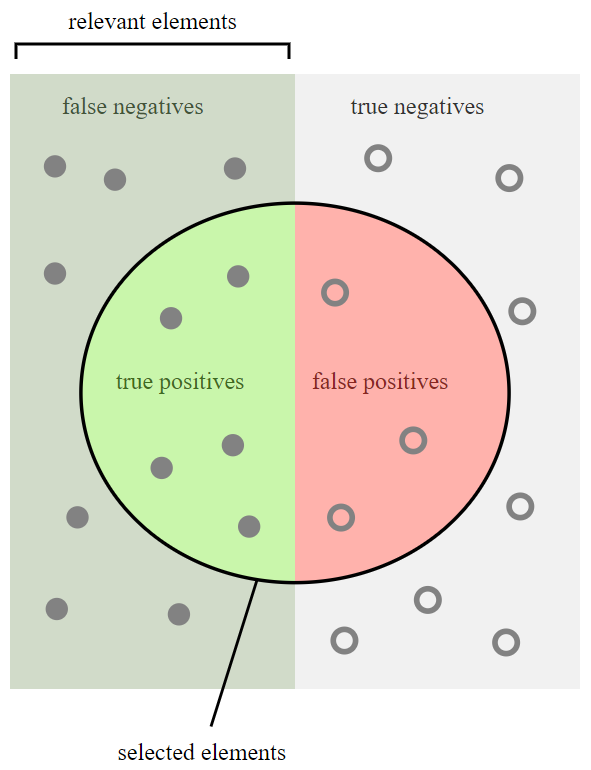
\includegraphics[scale=0.4]{metrics-overview}}
\caption{Overview about possible classification outcomes\cite{wiki01}}
\label{fig:metrics}
\end{figure}

For every binary classification task there exist exactly four possible outcomes. When the model classifies an element correctly it's either a \emph{true positive} or a \emph{true negative} value. The keyword true relates to the prediction the model did. Vice versa it's either a \emph{false positive} or a \emph{false negative} value if the model's prediction is wrong.

The combination of \emph{true positive} and \emph{false negative} values is the amount of relevant data we want to have a closer look at. For example this could be a set of named entities or a group of patients which have a certain disease.

\subsection{Why Accuracy is not enough}
\label{chap:accuracy}
Probably the most well-known and certainly the easiest metric to understand is called \emph{accuracy}. It describes the
closeness of a set of predictions to its corresponding \emph{truth values}. Accuracy is the proportion of all correctly classified
elements in relation to the total quantity. It's value lies somewhere between zero and one.

\begin{equation}
    \label{math:accuracy}
    accuracy = \frac{\textit{true positives} + \textit{true negatives}}{\textit{total population}}
\end{equation}

There is one large downside with accuracy which makes it useless for many classification problems. If there's one category
representing the majority of elements, accuracy will always be at a very high level. This is called an \emph{imbalanced
classification problem} \cite{koehrsen}. Imagine a model for detecting very rare diseases which simply labels each tested patient
as \emph{negative}. If the chance of getting this disease is about \(\frac{1}{10000}\), the accuracy of such model would be at
stunning $99.99\%$. That's why every data scientist should consider using more advanced metrics as described in the next section.

\subsection{Precision and Recall}

\emph{Precision} measures the accuracy of the positive predictions. In other words, it's the proportion of correctly classified
elements in relation to all elements the model marked as \emph{positive}. A model which classifies only one single element as
\emph{positive} (the rest as \emph{negative}) and is right about that, will have a \emph{precision} of $1.0$. The results of a
model with a high \emph{precision} are very useful because most values have been correctly classified and therefore can be used
for further processing.

\begin{equation}
    \label{math:precision}
    precision = \frac{\textit{true positives}}{\textit{true positives} + \textit{false positives}}
\end{equation}

\emph{Recall}, or sometimes called \emph{sensitivity}, is the number of correct classifications compared to the number of elements
which should have been found in total. A \emph{recall} of $100\%$ can simply be achieved by classifying every element as \emph{positive}.
Therefore it should be combined with \emph{precision} to get an expressive statement about the model performance.

\begin{equation}
    \label{math:recall}
    recall = \frac{\textit{true positives}}{\textit{true positives} + \textit{false negatives}}
\end{equation}

There is a trade-off between the two metrics \emph{precision} and \emph{recall}. An optimization which increases the \emph{recall}
will likely decrease the \emph{precision} and vice versa. If neither \emph{recall} nor \emph{precision} is more important, there
exists the \emph{F1 score} (\ref{math:f1}) which is the harmonic mean of both. The mean itself isn't very meaningful because if the
model performs very good at one metric and poorly at the other, it will be still around $0.5$. The harmonic mean punishes low values
and doesn't compensate them with high values for the opposite metric. In many cases, \emph{F1 score} is a good metric to describe the
overall performance of a model \cite{Grus15}.

\begin{equation}
    \label{math:f1}
    \textit{f1 score} = 2 * \frac{precision * recall}{precision + recall}
\end{equation}

